% !TeX spellcheck = en_GB

\documentclass[]{beamer}

\usepackage[utf8]{inputenc}
\usepackage[english]{babel}
\usepackage{tabularx}

\usetheme[titleformat=allsmallcaps, numbering=fraction, background=light, progressbar=frametitle]{metropolis}


\title{Computing Infrastructures}
\subtitle{Exercises on Queuing Network Model Inputs and Outputs}

\author{Stefano Cereda \\ stefano.cereda@polimi.it
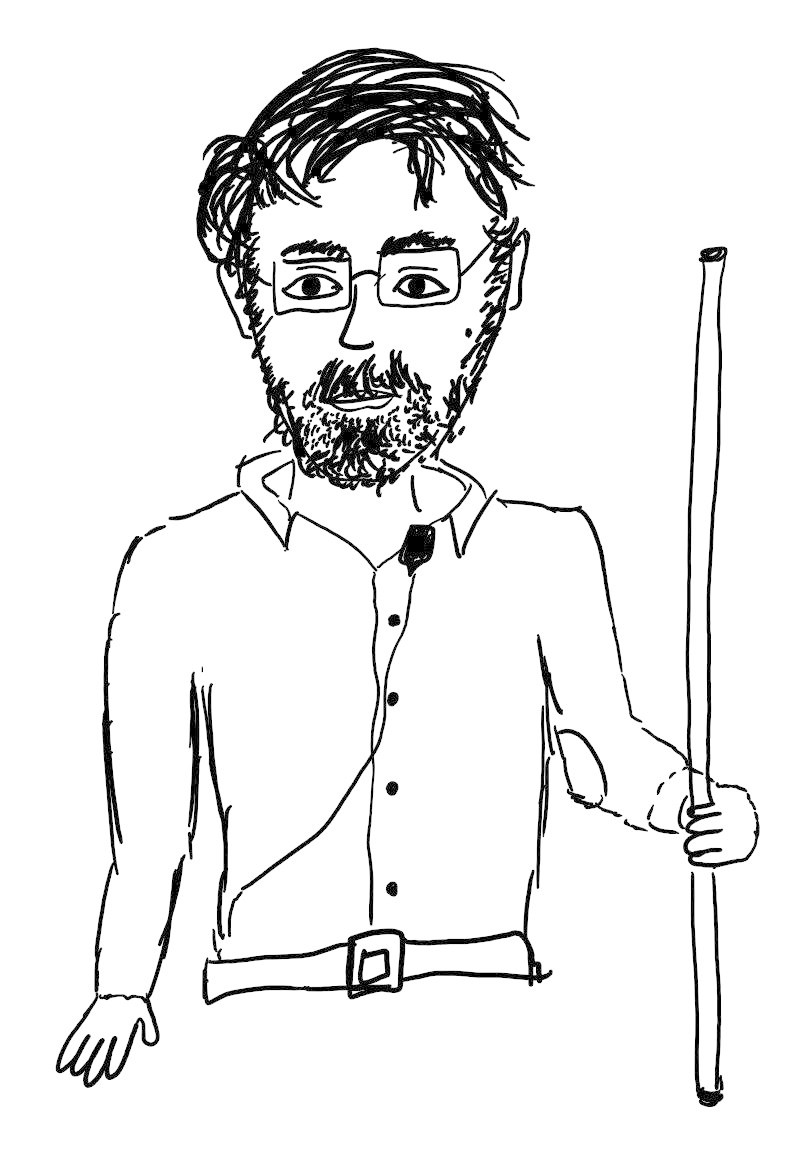
\includegraphics[width=0.1\linewidth]{../you_light}}

\date{13/05/2019}
\institute[PoliMi]{\vspace{0.5cm}Politecnico di Milano}
\logo{\includegraphics[width=10mm]{../logopolimi_dark}}

\setbeamercovered{invisible}

\makeindex

\begin{document}
\begin{frame}
	\maketitle
\end{frame}

\begin{frame}
    \huge{\alert{Tomorrow's lesson will start at 12.15}}
\end{frame}

\begin{frame}{Recap - Inputs}
\begin{itemize}
	\item Customers are described with \emph{workload intensity}:
	\begin{itemize}
		\item the \emph{arrival rate} $\lambda$ for \emph{transaction} workloads
		\item the \emph{population} $N$ for \emph{batch} workloads
		\item $N$ and the \emph{think time} $Z$ for \emph{terminal} workloads
	\end{itemize}
	\item Each service k is described with its type:
	\begin{itemize}
		\item Queuing
		\item Delay
	\end{itemize}
	\item The demand at each service is described with its \emph{service demand}: $D_k = V_kS_k$
\end{itemize}
\end{frame}

\begin{frame}{Recap - Outputs}
\begin{itemize}
	\item System Measures:
	\begin{itemize}
		\item average system response time: $R$
		\item system throughput: $X$
		\item average number in system: $Q$
	\end{itemize}
	\item Center Measures:
	\begin{itemize}
		\item utilization of center $k$: $U_k$
		\item average residence time at center $k$: $R_k$
		\item throughput of center $k$: $X_k$
		\item average queue length of center $k$: $Q_k$
	\end{itemize}
\end{itemize}
\end{frame}

% da tde 5/7/13
\begin{frame}{Exercise 1}
By monitoring a single class interactive system, we are able to measure the following data:
\begin{itemize}
	\item Disk demand: 4 seconds/transaction
	\item CPU demand: 1 seconds/transaction
	\item CPU utilization: 80\%
	\item Response time: 20 seconds/transaction
	\item Monitoring period: 6 minutes
	\item Number of users: 16
\end{itemize}
Which is the average think time of these users?
\end{frame}

\begin{frame}{Solution}
$$D_d = 4 \frac{sec}{tr} \quad D_c = 1 \frac{sec}{tr} \quad U_c = 0.8 \quad$$
$$R = 20 \frac{sec}{tr} \quad T = 6' \quad N = 16 \quad Z=?$$

$$Z = \frac{N}{X} - R \quad X?$$
$$X = \frac{U_c}{D_c} = \frac{0.8}{1\frac{sec}{tr}} = 0.8 \frac{tr}{sec}$$
$$Z = \frac{16}{0.8\frac{tr}{sec}} - 20 \frac{sec}{tr} = 0 \frac{sec}{tr}$$
\end{frame}

% da tde 5/7/13
\begin{frame}{Exercise 2}
Consider the following measurement data for an interactive system:
\begin{itemize}
	\item Measurement interval: 2 minutes
	\item number of users: 15
	\item average response time per transaction: 10 seconds
	\item Disk demand: 0.5 seconds/transaction
	\item CPU demand: 0.2 seconds/transaction
	\item Number of servers: 20
	\item Number of completed transactions: 60
\end{itemize}
On average, how many users are thinking?
\end{frame}

\begin{frame}{Solution}
$$N = N_{think} + N_{insystem} = N'+N'' \qquad N'=?$$

$$N' = N-N''$$
$$N'' = X\cdot R$$
$$X=\frac{C}{T}=0.5\frac{tr}{sec}$$
$$N''=0.5\cdot 10 = 5$$
$$N' = 15-5 = 10$$
\end{frame}

% da tde 5/7/13
\iffalse
\begin{frame}{Exercise 3}
Consider a multi class system with two classes of transactions. We have the following information about the system:
\begin{itemize}
	\item Class 1 response time: 4 seconds
	\item Class 2 response time: 1 seconds
	\item Class 1 throughput: 2 transactions/second
	\item Class 2 throughput: 4 transactions/second
\end{itemize}
Which is the average response time of the system?
\end{frame}

\begin{frame}{Solution}
$$R=\frac{R_1\cdot X_1}{X} + \frac{R_2\cdot X_2}{X}$$
$$X=X_1+X_2=6$$
$$R=\frac{6+1}{6} = \frac{10}{6}$$
\end{frame}
\fi

%da Ese 01 - Performance.pdf (ese.3)
\begin{frame}{Exercise 4}
In a batch system, a specific disk is performing, on average, 12 operation per second. We know that each batch transaction requires, on average, 6 accesses to this disk. Another disk in the system is handling 18 operations per second. Which is the average number of accesses to this second disk require by every batch transaction?
\end{frame}

\begin{frame}{Solution}
$$X_{D1} = 12 \quad V_{D1}=6 \quad X_{D2}=18$$

$$V_{D2} = \frac{X_{D2}}{X} = \frac{X_{D2}}{\frac{X_{D1}}{V_{D1}}} = \frac{18}{\frac{12}{6}} = 9$$
\end{frame}

%da performance evaluation.pdf (1)
\begin{frame}{Exercise 5}
The storage server of an intranet consists of two groups of disks, A and B, each having service times with means $S_A$ = 5ms and $S_B$ = 3ms. The mean number of visits for the two
components are $V_A$ = 20 and $V_B$ = 30. The throughput of A is 150 op./sec. The above data were collected
when the system is processing a workload generated by 300 users with think time $Z$ = 15 sec.

\begin{enumerate}
	\item Compute the System Throughput $X$ and the Utilization of B.
	\item Compute the system response time.
	\item If the number of users increases to 400, which will be the new response time?
\end{enumerate}
\end{frame}

\begin{frame}{Solution 1}
$$X = \frac{U_A}{D_A}$$
$$U_A = X_A \cdot S_A = 5 \frac{ms}{op} \cdot 150 \frac{op}{sec} = 75\%$$
$$D_A = V_A \cdot S_A = 20 \cdot 5ms = 100ms$$
$$X = \frac{0.75}{0.1} = 7.5\frac{op}{sec}$$

$$U_B = X \cdot D_B = X \cdot (S_B \cdot V_B) = 7.5 \cdot (3ms \cdot 30) = 7.5 \cdot 0.09 \frac{sec}{op} = 67.5\%$$
\end{frame}

\begin{frame}{Solution 2 and 3}
$$R = \frac{N}{X}-Z = \frac{300 op}{7.5 \frac{op}{sec}} -15 sec = 25 sec$$

\vspace{2cm}
We cannot say anything for $N=400$
\end{frame}


%da performance evaluation.pdf (3)
\begin{frame}{Exercise 6}
The throughput of a disk is 100 I/O operations per second. To complete a given request 20 visits to the disk
are required. The number of users is 100 and the response time is 15 seconds.

Compute the users think time.
\end{frame}

\begin{frame}{Solution}
$$Z = \frac{N}{X}-R$$
$$X = \frac{X_D}{V_D} = 5 \frac{op}{sec}$$
$$Z = \frac{100}{5} - 15 = 5 sec$$
\end{frame}

%da performance evaluation.pdf (5)
\begin{frame}{Exercise 7}
A web server of a company is connected to an intranet and is accessed by the employees that work
internally in the company resulting in a population of fixed size: $N$=21 users. The average think time of the
users is $Z$=20 sec. A complete execution of a request generates a load of $V_s$ = 20 operations to a specific
storage device whose utilization is $U_s$ = 0.30. The service time of the storage device per each visit is $S_s$ = 0.025
sec.

\begin{enumerate}
\item Determine the average system response time $R$
\item Compute the average throughput and system response time with $N$=40 users.
\end{enumerate}
\end{frame}

\begin{frame}{Solution}
$$R = \frac{N}{X} - Z$$
$$X = \frac{U_S}{D_S} = \frac{0.3}{V_S}{S_S} = \frac{0.3}{20 \cdot 0.025 sec} = 0.6 \frac{op}{sec}$$
$$R = \frac{21}{0.6} - 20 = 15 sec$$

We cannot say anything for $N=40$ 
\end{frame}

%da operational analysis ... (1)
\begin{frame}[allowframebreaks]{Exercise 8}
On a system with 3 disks, the following measurements were made:
\begin{itemize}
	\item throughput of each disk is 40 request/seconds ($X_{disk} = 40r/s$)
	\item 4 customers, on average, are either in queue or in service on each disk ($N_{disk+queue} = 4$)
	\item average think time is 5 seconds ($Z = 5s$)
	\item the service time on each disk is 0.0225 seconds ($S_{disk} = 0.0225s$)
\end{itemize}

\begin{enumerate}
	\item calculate the utilization of one disk without considering its queue.
	\item calculate the average time spent by each request in each disk, both in queue and
	in service.
	\item calculate the average number of users in service and the average number of users
	awaiting service.
	\item calculate the number of interactions per second, considering that the system-level
	average response time is 15 seconds and there are 7.5 active (i.e., non-thinking)
	users.
	\item calculate the total number of users.
\end{enumerate}
\end{frame}

\begin{frame}{Solution}
$D$ indicates just the disk, $Q$ is the queue and $D+Q$ the disk with its queue. Notice that $X_D = X_Q$ and that when we look at the disk+queue subsystem we have $R_D=S_D$.

$$U_D = X_D \cdot S_D = 90\%$$
$$R_{D+Q} = \frac{N_D}{X_D} = \frac{4}{40} = 0.1 sec$$

$$N_Q = X_D \cdot R_Q = X_D \cdot (R_{D+Q} - R_D) = 3.1$$
$$N_D = X_D \cdot R_D = 0.9 = U_D$$

$$X = \frac{N_{active}}{R} = \frac{7.5}{15} = 0.5 \frac{int}{sec}$$
$$N = X(R+Z) = 0.5(15+5)=10$$
\end{frame}

%da operational analysis ... (2)
\begin{frame}[allowframebreaks]{Exercise 9}
On the system depicted below, the following measurements were made:
\begin{itemize}
	\item average number of users is 23
	\item average response time as perceived by a user is 30 seconds
	\item throughput is 0.45 interactions/second
	\item average number of requests in memory (box 2) is 1.9
	\item average CPU service demand per interaction is 0.63 seconds
\end{itemize}


\begin{figure}
	\centering
	\includegraphics[width=0.7\linewidth]{system_t}
\end{figure}

\begin{enumerate}
	\item What is the average think time of a user?
	\item how many users are attempting to obtain service and how many of them are instead thinking?
	\item how much time elapses between the acquisition of memory and the completion of an interaction?
	\item what is the utilization of the CPU?
\end{enumerate}
\end{frame}

\begin{frame}{Solution}
$$N=23 \quad R=30sec \quad X=0.45 \frac{int}{sec} \quad N_{mem} = 1.9 \quad D_{cpu} = 0.63 sec$$

$Z = ?$ in box 4 $Z=\frac{N}{X}-R = \frac{23}{0.45}-30 = 21 sec$

$N_{think}? \quad N_{queue}?$ $N_q = N{notThink} - N_{mem} = X\cdot R - 1.9 = 0.45\cdot 30 - 1.9 = 11.6$ $N_{think} = N - N_{notThink} = N - 13.5 = 9.5$

$? = R_{box2} = \frac{N_{mem}}{X} = \frac{1.9}{0.45} = 4.2 sec >> (R-4.2)$ most time is spent in queue.

$U_{cpu} = X \cdot D_{cpu} = 0.45 \cdot 0.63 = 0.28 << 1$ the cpu has a very low usage as the system is limited by the memory queue. 
\end{frame}

\begin{frame}{Routing probabilities}
Consider the following open network, where $a$ and $b$ are routing probabilities. 
Which is the number of visits at station 1 and 2?\\
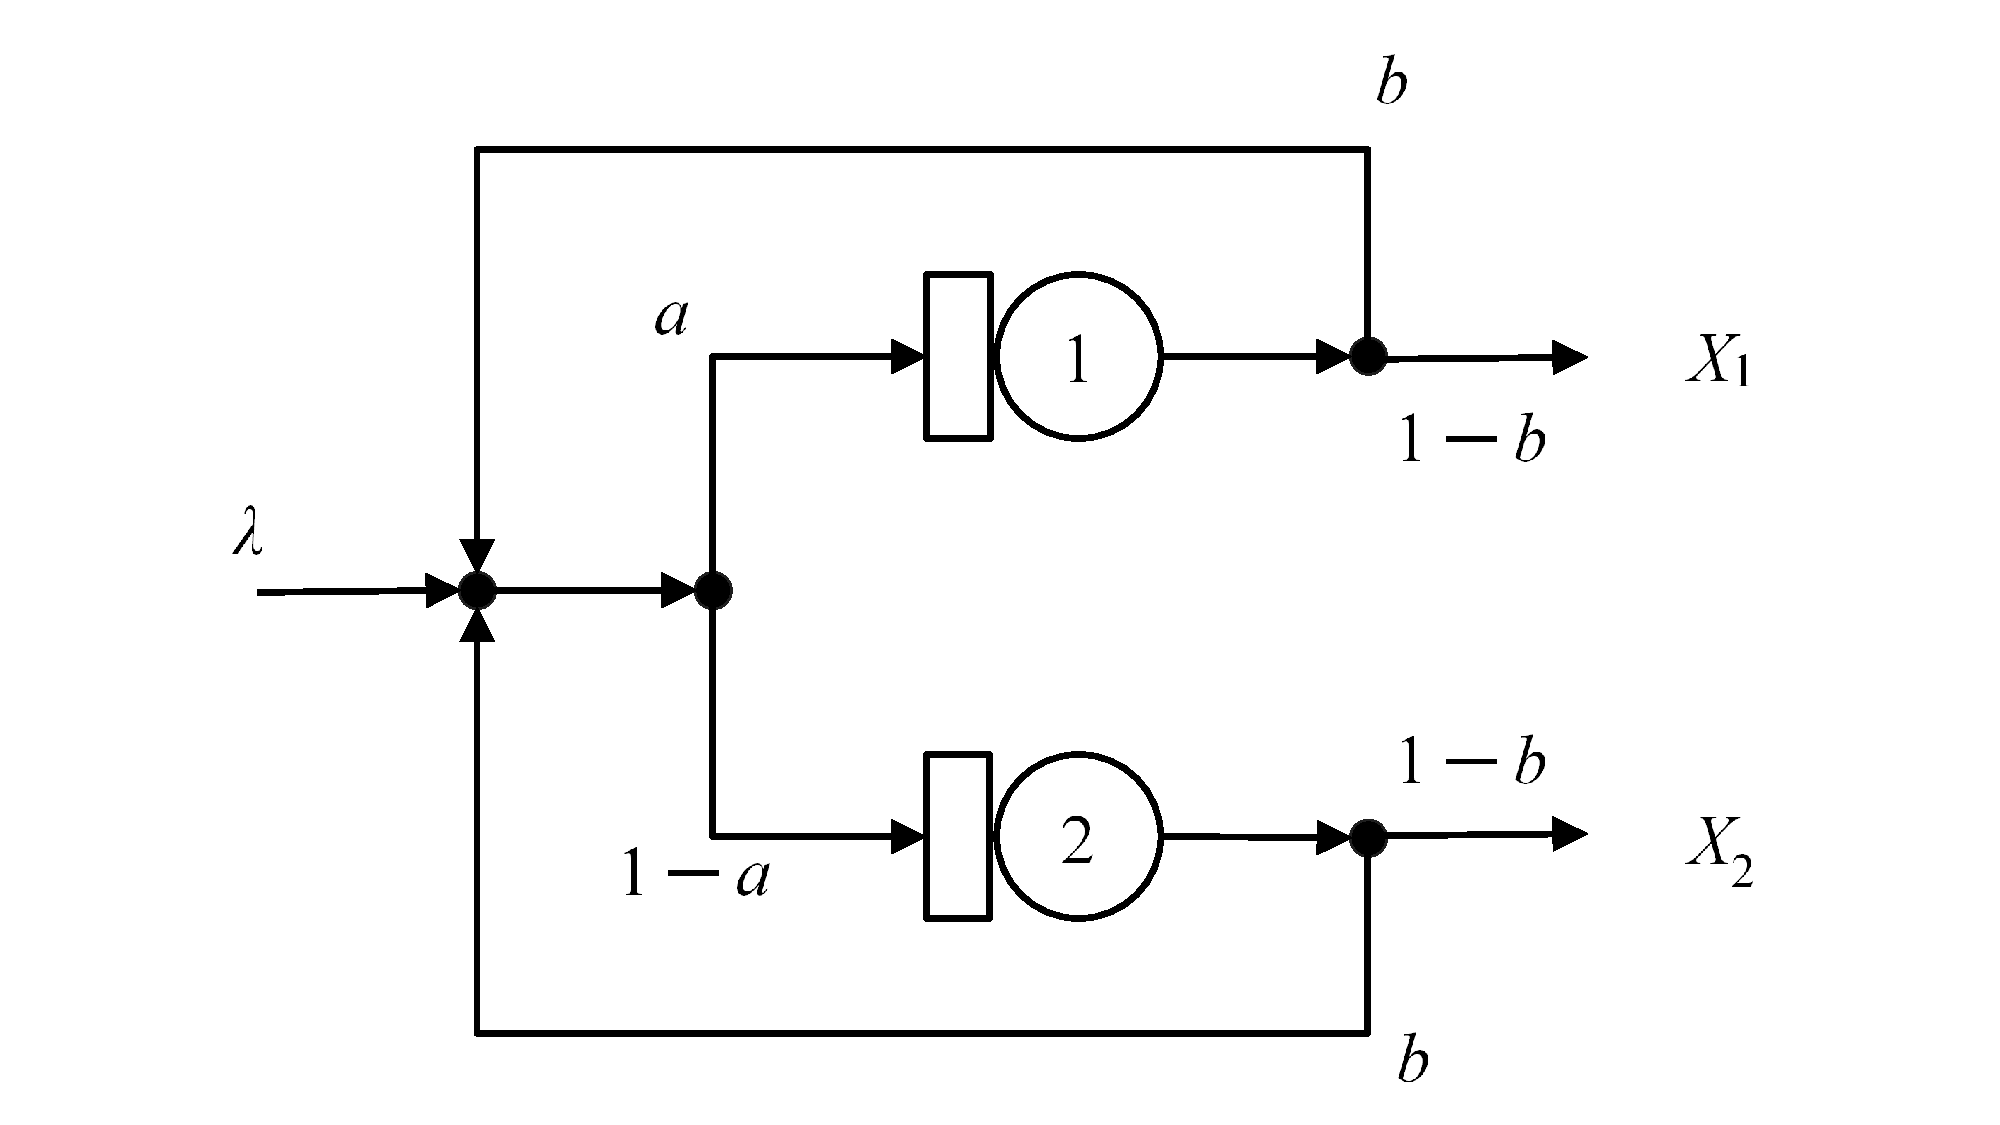
\includegraphics[width=0.6\linewidth]{./open1.png}
\end{frame}

\begin{frame}{Solution}
\[V_1 = a  (1 + b  V_1 + b  V2) = a  (1 + b  (V_1+V_2))\]
\[V_2 = (1-a)(1+ b V-1+ b V_2)\ = (1-a)(1+b(V_1+V_2)) \]
\[\frac{V_2}{V_1} = \frac{1-a}{a}\]
\[V_2 = V_1 \frac{1-a}{a} = \frac{V_1}{a} - \frac{a V_1}{a}\]
\[V_1 = a(1+b(V_1+\frac{V1}{a}-V_1)) = a + \frac{a b V_1}{a} \]
\[V_1 = \frac{a}{1-b}\]
\[V_2 = \frac{V_1}{a} - V_1 = \frac{1}{1-b} - \frac{a}{1-b} = \frac{1-a}{1-b}\]
\end{frame}

\begin{frame}{Routing probabilities}
Consider the following open network, where $a$ and $b$ are routing probabilities. 
Which is the number of visits at station 1, 2 and 3?\\
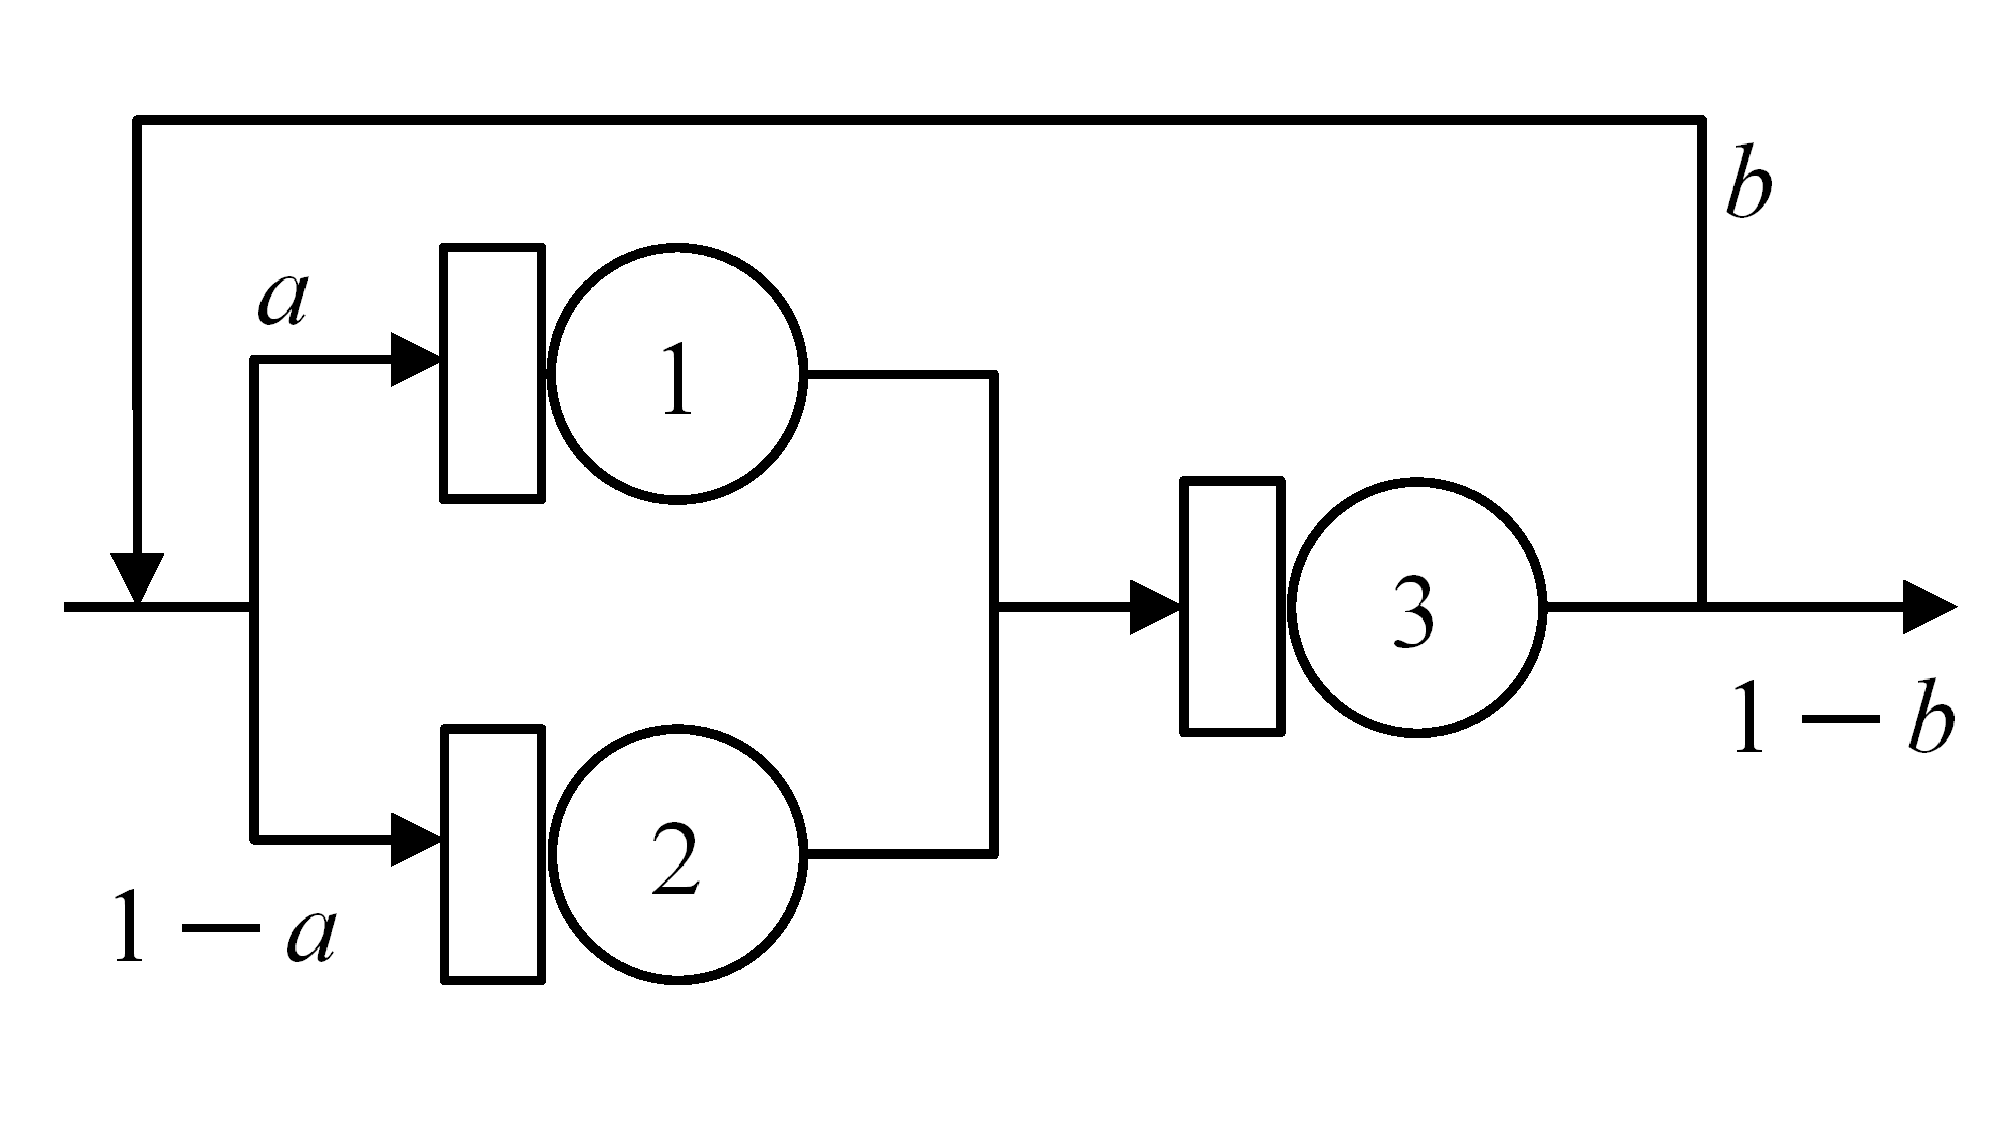
\includegraphics[width=0.6\linewidth]{./open2.png}
\end{frame}

\begin{frame}{Solution}
\[ V_1 = a (b V_3 +1)\]
\[V_2 = (1-a) (bV_3+1)\]
\[V_3 = V1+V2 = 1+bV_3 = \frac{1}{1-b}\]
\[V_1 = \frac{ab}{1-b} + a = \frac{a-ab+ab}{1-b} = \frac{a}{1-b} \]
\[V_2 = \frac{(1-a)b}{1-b} + \frac{(1-a)(1-b)}{1-b} = \frac{b - ab + 1 -a -b +ab}{1-b} = \frac{1-a}{1-b} \]
\end{frame}

\end{document}
